\subsection{Multiplier Comparison}

With the different multiplication algorithms, there is an underlying assumption regarding their performance. The more
advanced algorithms use fewer additions, which should - in theory - be quicker. However, there might be other things
to take into account, such as pre-computations and other overhead.

To determine which algorithm is actually the fastest for use in OpenECC, all of them are tested. The test performs a
full  encryption of a string, involving all layers of the software. A hundred tests are run
per algorithm, and the average time spent is recorded. The tests are run on a computer with an Intel Core i3 processor.

\begin{figure}[htb!]
	\centering
	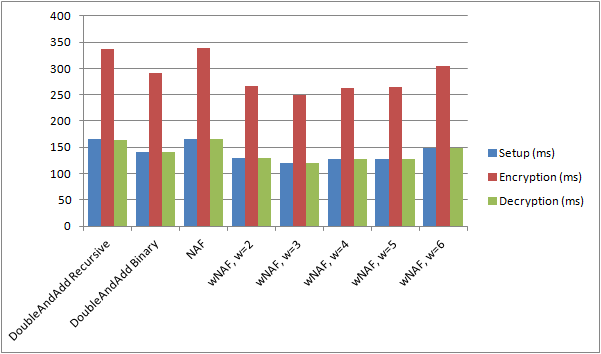
\includegraphics[width=\textwidth]{performance/multipliers-comparison}
	\caption{Comparison of differnt multiplication algorithms. wNAF with a window size of 3 is the fastest on average,
		having run each algorithm 100 times.}
	\label{fig:multipliers-comparison}
\end{figure}

Most of the algorithms do not have modifiable parameters, but the wNAF algorithm has a variable window size \(w\). For
this reason, the wNAF algorithm has been tested with a variety of window sizes, to determine which is the best.

The Double-and-Add algorithm has been implemented in both a recursive fashion (where it repeatedly calls itself, causing
overhead), and a binary-based version (where there is a slight overhead involved with finding the binary representation
of the number).

\(wNAF_3\) is found to be the fastest of the algorithms (full encryption of the string \texttt{"Hello, World."} takes an
average of \(491 \text{ ms}\).), and is selected as the default multiplier for all points. It is
interesting to note that the NAF algorithm is slower than Double-and-Add algorithm (as fewer additions should theoretically
be performed), which is probably to the overhead of creating the NAF form.